% Options for packages loaded elsewhere
% Options for packages loaded elsewhere
\PassOptionsToPackage{unicode}{hyperref}
\PassOptionsToPackage{hyphens}{url}
\PassOptionsToPackage{dvipsnames,svgnames,x11names}{xcolor}
%
\documentclass[
  letterpaper,
  DIV=11,
  numbers=noendperiod]{scrartcl}
\usepackage{xcolor}
\usepackage{amsmath,amssymb}
\setcounter{secnumdepth}{5}
\usepackage{iftex}
\ifPDFTeX
  \usepackage[T1]{fontenc}
  \usepackage[utf8]{inputenc}
  \usepackage{textcomp} % provide euro and other symbols
\else % if luatex or xetex
  \usepackage{unicode-math} % this also loads fontspec
  \defaultfontfeatures{Scale=MatchLowercase}
  \defaultfontfeatures[\rmfamily]{Ligatures=TeX,Scale=1}
\fi
\usepackage{lmodern}
\ifPDFTeX\else
  % xetex/luatex font selection
\fi
% Use upquote if available, for straight quotes in verbatim environments
\IfFileExists{upquote.sty}{\usepackage{upquote}}{}
\IfFileExists{microtype.sty}{% use microtype if available
  \usepackage[]{microtype}
  \UseMicrotypeSet[protrusion]{basicmath} % disable protrusion for tt fonts
}{}
\makeatletter
\@ifundefined{KOMAClassName}{% if non-KOMA class
  \IfFileExists{parskip.sty}{%
    \usepackage{parskip}
  }{% else
    \setlength{\parindent}{0pt}
    \setlength{\parskip}{6pt plus 2pt minus 1pt}}
}{% if KOMA class
  \KOMAoptions{parskip=half}}
\makeatother
% Make \paragraph and \subparagraph free-standing
\makeatletter
\ifx\paragraph\undefined\else
  \let\oldparagraph\paragraph
  \renewcommand{\paragraph}{
    \@ifstar
      \xxxParagraphStar
      \xxxParagraphNoStar
  }
  \newcommand{\xxxParagraphStar}[1]{\oldparagraph*{#1}\mbox{}}
  \newcommand{\xxxParagraphNoStar}[1]{\oldparagraph{#1}\mbox{}}
\fi
\ifx\subparagraph\undefined\else
  \let\oldsubparagraph\subparagraph
  \renewcommand{\subparagraph}{
    \@ifstar
      \xxxSubParagraphStar
      \xxxSubParagraphNoStar
  }
  \newcommand{\xxxSubParagraphStar}[1]{\oldsubparagraph*{#1}\mbox{}}
  \newcommand{\xxxSubParagraphNoStar}[1]{\oldsubparagraph{#1}\mbox{}}
\fi
\makeatother


\usepackage{longtable,booktabs,array}
\usepackage{calc} % for calculating minipage widths
% Correct order of tables after \paragraph or \subparagraph
\usepackage{etoolbox}
\makeatletter
\patchcmd\longtable{\par}{\if@noskipsec\mbox{}\fi\par}{}{}
\makeatother
% Allow footnotes in longtable head/foot
\IfFileExists{footnotehyper.sty}{\usepackage{footnotehyper}}{\usepackage{footnote}}
\makesavenoteenv{longtable}
\usepackage{graphicx}
\makeatletter
\newsavebox\pandoc@box
\newcommand*\pandocbounded[1]{% scales image to fit in text height/width
  \sbox\pandoc@box{#1}%
  \Gscale@div\@tempa{\textheight}{\dimexpr\ht\pandoc@box+\dp\pandoc@box\relax}%
  \Gscale@div\@tempb{\linewidth}{\wd\pandoc@box}%
  \ifdim\@tempb\p@<\@tempa\p@\let\@tempa\@tempb\fi% select the smaller of both
  \ifdim\@tempa\p@<\p@\scalebox{\@tempa}{\usebox\pandoc@box}%
  \else\usebox{\pandoc@box}%
  \fi%
}
% Set default figure placement to htbp
\def\fps@figure{htbp}
\makeatother


% definitions for citeproc citations
\NewDocumentCommand\citeproctext{}{}
\NewDocumentCommand\citeproc{mm}{%
  \begingroup\def\citeproctext{#2}\cite{#1}\endgroup}
\makeatletter
 % allow citations to break across lines
 \let\@cite@ofmt\@firstofone
 % avoid brackets around text for \cite:
 \def\@biblabel#1{}
 \def\@cite#1#2{{#1\if@tempswa , #2\fi}}
\makeatother
\newlength{\cslhangindent}
\setlength{\cslhangindent}{1.5em}
\newlength{\csllabelwidth}
\setlength{\csllabelwidth}{3em}
\newenvironment{CSLReferences}[2] % #1 hanging-indent, #2 entry-spacing
 {\begin{list}{}{%
  \setlength{\itemindent}{0pt}
  \setlength{\leftmargin}{0pt}
  \setlength{\parsep}{0pt}
  % turn on hanging indent if param 1 is 1
  \ifodd #1
   \setlength{\leftmargin}{\cslhangindent}
   \setlength{\itemindent}{-1\cslhangindent}
  \fi
  % set entry spacing
  \setlength{\itemsep}{#2\baselineskip}}}
 {\end{list}}
\usepackage{calc}
\newcommand{\CSLBlock}[1]{\hfill\break\parbox[t]{\linewidth}{\strut\ignorespaces#1\strut}}
\newcommand{\CSLLeftMargin}[1]{\parbox[t]{\csllabelwidth}{\strut#1\strut}}
\newcommand{\CSLRightInline}[1]{\parbox[t]{\linewidth - \csllabelwidth}{\strut#1\strut}}
\newcommand{\CSLIndent}[1]{\hspace{\cslhangindent}#1}



\setlength{\emergencystretch}{3em} % prevent overfull lines

\providecommand{\tightlist}{%
  \setlength{\itemsep}{0pt}\setlength{\parskip}{0pt}}



 


\KOMAoption{captions}{tableheading}
\makeatletter
\@ifpackageloaded{caption}{}{\usepackage{caption}}
\AtBeginDocument{%
\ifdefined\contentsname
  \renewcommand*\contentsname{Table of contents}
\else
  \newcommand\contentsname{Table of contents}
\fi
\ifdefined\listfigurename
  \renewcommand*\listfigurename{List of Figures}
\else
  \newcommand\listfigurename{List of Figures}
\fi
\ifdefined\listtablename
  \renewcommand*\listtablename{List of Tables}
\else
  \newcommand\listtablename{List of Tables}
\fi
\ifdefined\figurename
  \renewcommand*\figurename{Figure}
\else
  \newcommand\figurename{Figure}
\fi
\ifdefined\tablename
  \renewcommand*\tablename{Table}
\else
  \newcommand\tablename{Table}
\fi
}
\@ifpackageloaded{float}{}{\usepackage{float}}
\floatstyle{ruled}
\@ifundefined{c@chapter}{\newfloat{codelisting}{h}{lop}}{\newfloat{codelisting}{h}{lop}[chapter]}
\floatname{codelisting}{Listing}
\newcommand*\listoflistings{\listof{codelisting}{List of Listings}}
\makeatother
\makeatletter
\makeatother
\makeatletter
\@ifpackageloaded{caption}{}{\usepackage{caption}}
\@ifpackageloaded{subcaption}{}{\usepackage{subcaption}}
\makeatother
\usepackage{bookmark}
\IfFileExists{xurl.sty}{\usepackage{xurl}}{} % add URL line breaks if available
\urlstyle{same}
\hypersetup{
  pdftitle={Regression Analysis of Seasonal Patterns in Vehicle Theft Data},
  pdfauthor={Kumari Shyama},
  colorlinks=true,
  linkcolor={blue},
  filecolor={Maroon},
  citecolor={Blue},
  urlcolor={Blue},
  pdfcreator={LaTeX via pandoc}}


\title{Regression Analysis of Seasonal Patterns in Vehicle Theft
Data\thanks{Project repository available at:
\url{https://github.com/shyamaku/MATH261A-project}.}}
\author{Kumari Shyama}
\date{September 24, 2025}
\begin{document}
\maketitle
\begin{abstract}
Every year, a significant number of vehicle theft reports are captured
by the Police Department in California, USA. In the year 2024, 7,250
vehicle thefts were reported in San Francisco. The project aims to
explore seasonal patterns of vehicle thefts in San Francisco throughout
the year using a Simple Linear Regression Model to understand if there
is any significant impact of summer, winter, or holiday seasons on the
number of thefts occurring. The analysis results suggests that there is
an overall decrease in thefts in the year 2024. Through the scatterplot,
patterns suggesting increase in theft in summer and a decrease in winter
are visible. However, there can be many various factors involved
affecting the decline; the regression model only explains approximately
33\% variation in the data.
\end{abstract}


\section{Introduction}\label{introduction}

In the United States, the issue of vehicle theft has significantly
impacted residents for many years. Incidents of stolen vehicles,
break-ins, and parts theft have been increasing rapidly. However, in
2024, San Francisco, California, saw its first significant decrease in
the number of such cases (Fang 2025). Many factors could have
contributed to the resource management and allocation for the San
Francisco Police Department (SFPD) for the same. While researchers often
emphasize the overall crime trend and spatial data for coming up with
theft prevention measures, there has been less emphasis on the seasonal
trend of vehicle thefts. Our initial assumption states that during
summer, there is a significant increase in people going out, thus
increasing the number of vehicles on the street. However, during peak
winters, there would be a decrease in vehicles on the road. This project
aims to study whether there is a significant impact on thefts based on
seasonal variations and holiday periods in the year 2024.

The project analyses trends using scatterplots and applies simple linear
regression to interpret the correlation between seasons and vehicle
theft. It also examines the limitations of the linear regression model
using the residual vs fitted plot. Through this study, the expectation
is to provide significant results with the aim of assisting the SFPD
with better resource allocations during those periods to further reduce
the crime rates. The remainder of this paper is structured as follows:
Section~\ref{sec-data} introduces the data used in this analysis
Section~\ref{sec-methods} describes the model\ldots{}

\section{Data}\label{sec-data}

The dataset used in the project is obtained from DataSF, which is an
open data portal (DataSF 2025). It is a reliable source of data as the
incidents are filed by officers and members of the public. Additionally,
it does not contain any confidential information related to the
incidents. The dataset contains 969,326 records of various incidents
(Fraud, Assault, Motor Vehicle Theft, etc.) captured from 2018 to the
present. Each row describes the date, time, year of an incident, along
with incident description, ID, category, police district, analysis
neighborhood, resolution, and other incident area-related fields.

For the scope of this analysis, the data has been filtered to include
only records of ``Motor Vehicle Theft'' for the year 2024. Since there
has been a recent decline in vehicle theft incidents in 2024, this
project aims to explore trends based on the lower number of crimes. From
the incident date field, the week of the year has been extracted, and
then records have been grouped by weeks to count the number of vehicle
thefts each week.

\begin{figure}

\centering{

\pandocbounded{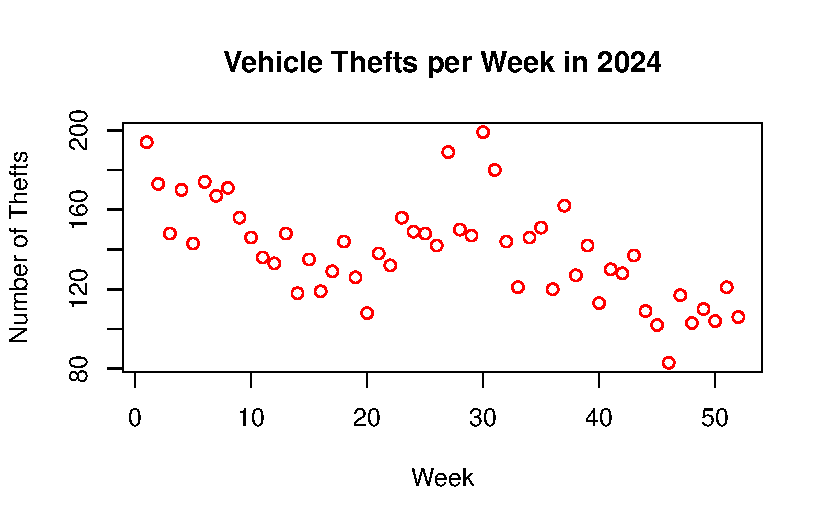
\includegraphics[keepaspectratio]{first_project_files/figure-pdf/fig-vehicle-theft-scatter-1.pdf}}

}

\caption{\label{fig-vehicle-theft-scatter}Scatter plot of week in x-axis
and number of thefts in y-axis.}

\end{figure}%

Figure~\ref{fig-vehicle-theft-scatter} indicates a negative linear
association between number of thefts and week.

\section{Methods}\label{sec-methods}

This project adopts the simple linear regression model with week of the
year as the predictor \(X_i\) and number of vehicle thefts as the
response \(Y_i\), where \(i = 1, 2, ..., n\) and \(n\) is the number of
records. The model can be represented with the following equation:

\[Y_i = \beta_0 +\beta_1 X_i + \varepsilon_i\]

In this model, \(\beta_1\) represents the slope, which describes the
change in the number of vehicle thefts as the week increases.
\(\beta_0\) represents the intercept, which describes the number of
vehicle thefts at week 0. and \(\epsilon\) represents the random error,
which describes the unexplained variation of data.

Next, after fitting the model as per the above equation, analysis of
variance is performed using ANOVA. Additionally, the project analyses
the model's fit using the residual values. Residuals are the difference
between observed and predicted values, written as,
\[e_i = Y_i - \hat{Y}\]

The analysis has been implemented using the R programming language (R
Core Team 2024) and packages including (Wickham et al. 2023),(Wickham
2016)

\section{Results}\label{sec-results}

The linear model fit for the number of vehicle thefts vs.~week is given
in the summary below:

\begin{verbatim}

Call:
lm(formula = num_theft ~ week, data = theft_per_week_2024)

Residuals:
    Min      1Q  Median      3Q     Max 
-37.717 -13.646  -2.054  10.781  63.029 

Coefficients:
            Estimate Std. Error t value Pr(>|t|)    
(Intercept) 164.5724     5.8788  27.994  < 2e-16 ***
week         -0.9534     0.1930  -4.939 9.17e-06 ***
---
Signif. codes:  0 '***' 0.001 '**' 0.01 '*' 0.05 '.' 0.1 ' ' 1

Residual standard error: 20.89 on 50 degrees of freedom
Multiple R-squared:  0.3279,    Adjusted R-squared:  0.3145 
F-statistic: 24.39 on 1 and 50 DF,  p-value: 9.175e-06
\end{verbatim}

The estimated slope parameter is \(b_1=\) -0.953. In other words, as the
weeks progress, there is a decrease in the number of vehicle thefts by
\(\approx 1\). The estimated intercept is \(b_0=\) 164.572 which
explains the expected number of thefts at week = 0. The R-squared value:
\(0.3279\) explains \(\approx 33\%\) of the variation in the theft
numbers per week.

\begin{verbatim}
Analysis of Variance Table

Response: num_theft
          Df Sum Sq Mean Sq F value    Pr(>F)    
week       1  10646 10646.5  24.393 9.175e-06 ***
Residuals 50  21823   436.5                      
---
Signif. codes:  0 '***' 0.001 '**' 0.01 '*' 0.05 '.' 0.1 ' ' 1
\end{verbatim}

Using ANOVA, the null hypothesis \(\beta_1=0\) is compared with the
two-sided alternative hypothesis \(\beta_1\not=0\). In order to reject
the null hypothesis, the mean squared regression (MSR) should be very
large compared to the mean squared error (MSE). In the above result, MSR
= \(10646.5\) \textgreater\textgreater{} MSE = \(436.5\). Thus, the null
hypothesis is rejected.

Figure~\ref{fig-vehicle-theft-scatter} indicates that the initial
assumptions hold value. Between week 23-37 (summer), there can be seen a
spike in the number of thefts, which falls under the earlier assumption
of this project. Similarly, week 45-55 (winter) shows the lowest number
of thefts in San Francisco.

\begin{figure}

\centering{

\pandocbounded{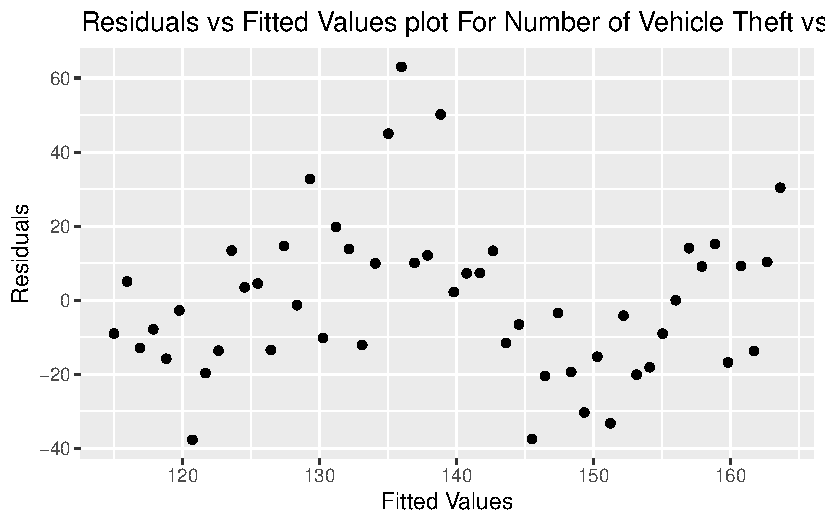
\includegraphics[keepaspectratio]{first_project_files/figure-pdf/fig-vehicle-residual-1.pdf}}

}

\caption{\label{fig-vehicle-residual}Scatter plot of fitted values
(x-axis) and residuals (y-axis) for a simple linear regression}

\end{figure}%

Figure~\ref{fig-vehicle-residual} examines the residuals to assess model
fit. From the scatterplot, the following can be interpreted: 1. The
regression function is linear as there are no visible arcs in the plot.
2. The error terms have equal variance, as there is no major spread in
the data points with the increase in weeks. 3. The error terms are not
completely independent, as we can see that residuals increase and
decrease with the increase in the fitted values. 4. The error terms are
not normally distributed.

\section{Discussion}\label{sec-discussion}

The analysis between vehicle thefts and week of the year 2024 explains a
few seasonal patterns in the data according to my research objective.
However, after assessing the residual vs fitted model plot, it can be
said that linear regression model doesn't necessarily fit the data.
Thus, the increasing and decreasing patterns of number of vehicle thefts
can be influenced by other factors and cannot be explained only using
the seasonal factors.

For further inspection of the assumptions made initially, the analysis
should be done with multiple years of data. This could provide trends of
number of vehicle thefts across weeks which would be helpful in
interpreting the results with better confidence. Additionally, the
results could change based on the time of day and police districts.

\section*{References}\label{references}
\addcontentsline{toc}{section}{References}

\phantomsection\label{refs}
\begin{CSLReferences}{1}{0}
\bibitem[\citeproctext]{ref-datasf_police_incidents}
DataSF. 2025. {``Police Department Incident Reports: 2018 to Present.''}
Police Department. \url{/url\%7Bhttps://data.sfgov.org/d/wg3w-h783\%7D}.

\bibitem[\citeproctext]{ref-CBS_News}
Fang, Tim. 2025. {``Car Thefts in California down 13\% Statewide, CHP
Says.''} CBS News.
\url{https://www.cbsnews.com/sanfrancisco/news/california-car-thefts-down-13pct-statewide-23-24-chp-says/}.

\bibitem[\citeproctext]{ref-R_language}
R Core Team. 2024. {``R: A Language and Environment for Statistical
Computing.''} Vienna, Austria: R Foundation for Statistical Computing.
\url{https://www.R-project.org/}.

\bibitem[\citeproctext]{ref-R_ggplot2}
Wickham, Hadley. 2016. \emph{Ggplot2: Elegant Graphics for Data
Analysis}. Springer-Verlag New York.
\url{https://ggplot2.tidyverse.org}.

\bibitem[\citeproctext]{ref-R_dplyr}
Wickham, Hadley, Romain François, Lionel Henry, Kirill Müller, and Davis
Vaughan. 2023. {``Dplyr: A Grammar of Data Manipulation.''}
\url{https://CRAN.R-project.org/package=dplyr}.

\end{CSLReferences}




\end{document}
